\documentclass[a4paper,10pt]{article}
\usepackage[vmargin=1.2cm, hmargin=1.5cm]{geometry}
\input{MySetup}
\usepackage{enumitem}
\setlist{nosep,leftmargin=*} 
\setlist[itemize]{topsep=2pt, partopsep=2pt, parsep=2pt}
\usepackage{tikz} % For circular photo

\begin{document}
\thispagestyle{empty}

%-------------------------------------------------------------------------------------------------------
% Left column
%-------------------------------------------------------------------------------------------------------
\begin{adjustbox}{valign=t}
\begin{minipage}[t]{0.3\textwidth}
\begin{center}
% Circular photo
\begin{tikzpicture}
    \node[circle, draw=ColorOne, line width=1.5pt, minimum size=3cm, inner sep=0pt, path picture={
        \node at (path picture bounding box.center){
            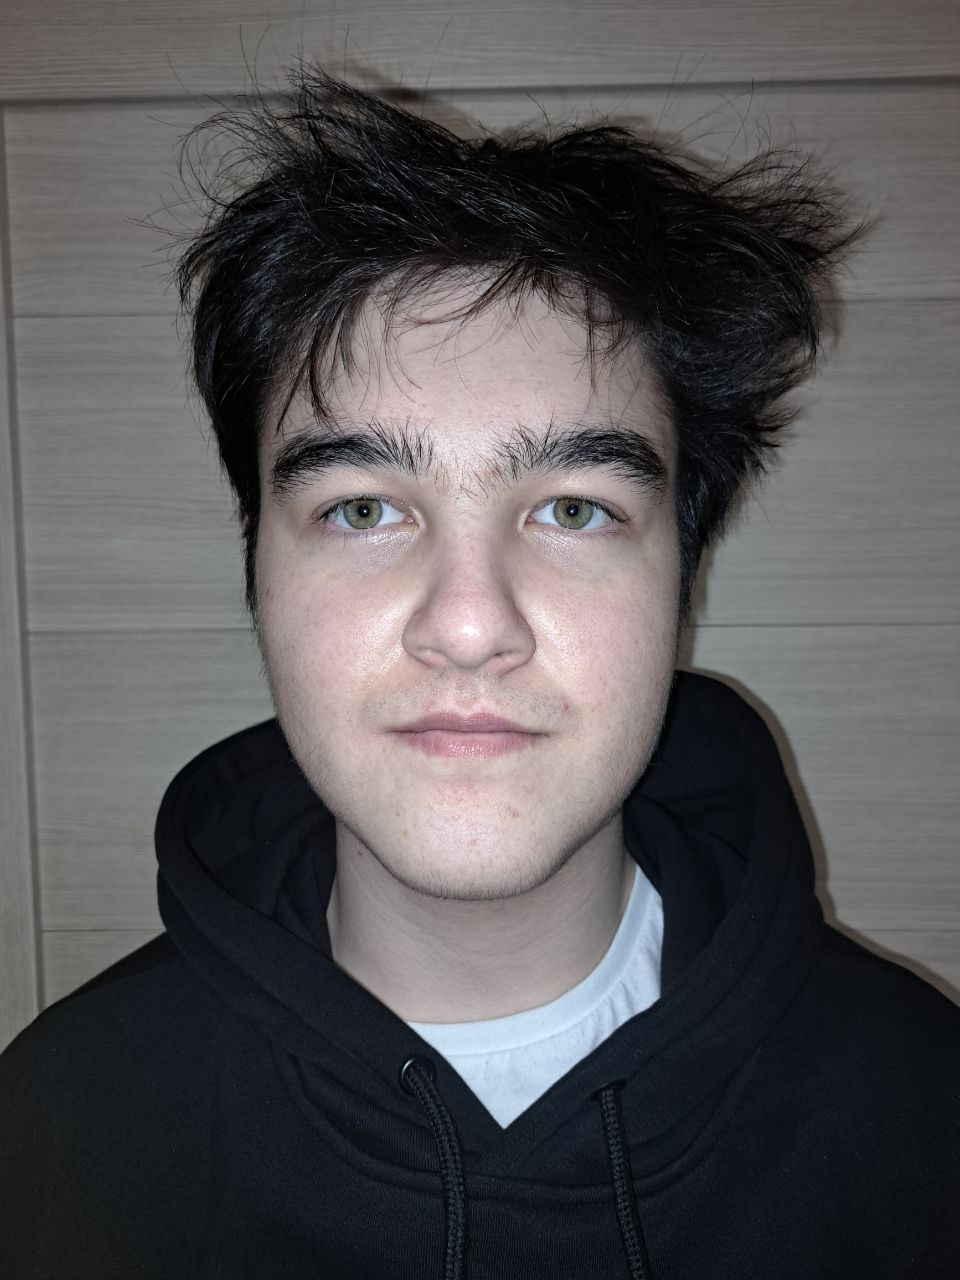
\includegraphics[width=3cm]{photo.jpg}
        };
    }] {};
\end{tikzpicture}

\vspace{0.3cm} % Space between photo and name

{\LARGE \bfseries Baidusenov Timur}

\vspace{0.2cm}

Born: September 20, 2005\\
Currently: Dolgoprudny, Russia\\

\vspace{0.2cm}

\textcolor{ColorTwo}{\faEnvelopeO} 
\myhref{mailto:baidiusenov.tb@phystech.edu}{baidiusenov.tb@phystech.edu} \\

\textcolor{ColorTwo}{Telegram:} 
\myhref{https://t.me/bai_tim}{@bai\_tim}
\end{center}

\vspace{-0.3cm}

%----------------------------------------------------
\section*{Scientific interests}
\raggedright
\textcolor{ColorOne}{$\circ$} C++, C\\
\textcolor{ColorOne}{$\circ$} Compiler technologies\\
\textcolor{ColorOne}{$\circ$} RISC-V

\vspace{-0.2cm}

%----------------------------------------------------
\section*{Education}
\vspace{-0.2cm}
\noindent
\textbf{MIPT DREC} \\
Dolgoprudny, Russia \\[1pt]
\textbf{Second-year student, Applied Mathematics and Physics} \\[1pt]
\textbf{GPA:} 8.9 / 10.0

\vspace{-0.2cm}

%----------------------------------------------------
\section*{Languages}
Russian - Native Proficiency\\
English - B2

\vspace{0.5cm}
\begin{center}
\myhref{https://github.com/baitim}{
    
\includegraphics[width=3cm]{qr-code.png}
}
\end{center}

\end{minipage}
\end{adjustbox}
%
%-------------------------------------------------------------------------------------------------------
% Vertical rule
%-------------------------------------------------------------------------------------------------------
\hfill
\begin{adjustbox}{valign=t}
\begin{minipage}{0.05\textwidth}
\MyVerticalRule
\end{minipage}
\end{adjustbox}
\hfill
%
%-------------------------------------------------------------------------------------------------------
% Right column
%-------------------------------------------------------------------------------------------------------
\begin{adjustbox}{valign=t}
\begin{minipage}[t]{0.6\textwidth}

%----------------------------------------------------
\section*{Learning Experience}
\begin{description}[leftmargin=!,labelwidth=2em]
\item[\textcolor{ColorOne}{2023-2024}] \textbf{System programming \& compiler technology course} \\ Huawei, Ilya Dedinsky's course
\item[\textcolor{ColorOne}{2024-2025}] \textbf{Basic course of programming in C++} \\ Yadro, Konstantin Vladimirov's course
\end{description}

%----------------------------------------------------
\section*{Technical Skills}
\vspace{-0.2cm}
\begin{tabular}{@{}l l@{}}
\textbf{Programming Languages:}     & C++, C, Python \\
\textbf{Development Tools:}         & Git, Linux, GDB, Assembly, \LaTeX\\
& Cmake, Conan, Docker, Github Actions\\
\textbf{Technologies \& Libraries:} & Google Test, OpenGL, OpenCL, Flex, Bison \\
\textbf{Hardware \& CAD:}           & SolidWorks, EasyEDA, ESP32
\end{tabular}

%----------------------------------------------------
\section*{Projects}
\vspace{-0.2cm}

\textbf{C++ Projects:}
\begin{itemize}
\item \myhref{https://github.com/baitim/ParaCL}{\textbf{ParaCL}} - Custom interpreted language with C/Python syntax. Frontend: Flex/Bison, AST generation, interpreter runtime

\item \myhref{https://github.com/baitim/TrianglesGL}{\textbf{TrianglesGL}} - OpenGL-based 3D visualization of triangle intersection algorithms. GPU-accelerated rendering with real-time transformations

\item \myhref{https://github.com/baitim/MatrixChain}{\textbf{MatrixChain}} - Optimized matrix chain multiplication using dynamic programming. Includes a custom memory-efficient matrix class

\item \myhref{https://github.com/baitim/BitonicSort}{\textbf{BitonicSort}} - OpenCL-accelerated bitonic sort implementation with comparative performance analysis. As a result, std::sort was outpaced.

\item \myhref{https://github.com/baitim/Graph}{\textbf{Graph}} - C++ graph theory library from TAOCP 7.2.1.6.S. implementing BFS, DFS, Bipartite with specific representation

\item \myhref{https://github.com/baitim/AVLTree}{\textbf{AVLTree}} - Self-balancing AVL tree implementation for segment queries. Supports insertion, deletion, and logarithmic time range queries

\item \myhref{https://github.com/baitim/Caches}{\textbf{Caches}} - Configurable cache simulator with LRU, LFU and ARC policies and hit/miss statistics

\item[] \small{\textit{All C++ projects implement CMake-based builds with Conan packaging deployed to \myhref{https://github.com/baitim/ConanPackages}{ConanPackages}. Components use internal packages from this registry.}}
\end{itemize}

\textbf{Hardware Projects:}
\begin{itemize}
\item \myhref{https://github.com/baitim/Drone}{\textbf{Drone}} - Team project developing a flying drone based on ESP32 microcontroller with integrated PID balancing
\end{itemize}

\end{minipage}
\end{adjustbox}
\end{document}